%\documentstyle[11pt,epsf]{article}
%\documentstyle[11pt,epsf]{report}
%\documentclass[11pt,epsf]{report}

%\documentclass[11pt]{article}
%\usepackage{epsfig}

\documentclass[10pt,dvips]{article}

\usepackage[dvips]{graphicx}
\usepackage[hang]{subfigure}


\pagestyle{myheadings}

% Some definitions I use in these instructions.

\def\emphasize#1{{\sl#1\/}}
\def\arg#1{{\it#1\/}}
\let\prog=\arg

\def\edcomment#1{\iffalse\marginpar{\raggedright\sl#1\/}\else\relax\fi}
\marginparwidth 1.25in
\marginparsep .125in
\marginparpush .25in
\reversemarginpar

\title{Using CMHOG with NEMO and MIRIAD}
\author{Peter Teuben}
% \affil{Astronomy Department, University of Maryland, College Park, MD 20742, USA}


\begin{document}

\maketitle


\begin{abstract}

An overview is given how to use and extend 
the Piner, Stone \& Teuben (1995, ApJ 449, 508) hydro code
{\tt cmhog}, and in particular how 
HDF\footnote{{\tt cmhog} only writes the HDF4/SDS data format, no HDF5!}
output data can be used with
NEMO and MIRIAD for some basic visualization and data analysis.
Only single runs are covered, restart runs are not discussed here.
An unfortuitous bug that combined a wrong bar position angle and reversed
the azimuthal forces from the bar was fixed in 2011, and updated
results are further discussed in Kim, Seo, Stone, Yoon \& Teuben (2011)

\end{abstract}

\section{Introduction}

The ``{\tt cmhog}'' code is an isothermal PPM code, 
that was adopted to run a 2-dimensional polar-grid gas flow in a 
barred galaxy (Piner, Stone \& Teuben, 1995 ApJ 449, 508).
Because of symmetry, only half of the plane is normally
simulated, with the appropriate  boundary condition.
The bar is elongated along the Y-axis, with 
counter clockwise gas flow. Initially the bar is absent, but
slowly (usually 0.1Gyr) turned on while keeping
the total mass constant. The simulation
is usually followed for 1-2 Gyr, to settle into a quasi-stationary
state, at which time the gas properties (density, flow velocities)
can be studied and compared to observations.

\section{The ``cmhogin'' input file}

The {\tt cmhog} program uses a classic, but not often used, method of parameter input
that is a little more rubust to errors than the more often (ab)used method
of reading information from standard input or some user defined file.
It's called {\tt namelist}\index{namelist},
a specially formatted textfile, 
and works roughly like magically reading a FORTRAN named common block.
in one read, with a convenient way to set defaults for all values
in the program.

\subsection{For the programmer}

For the programmer it is very convenient to pass parameters via a namelist.
After opening the unit somewhere at the beginning of the program
(cmhog does this in {\tt mstart.src}) various subroutines can simply read
the namelist  that they need with a simple read statement.

\begin{verbatim}
    open(unit=1,file='cmhogin' ,status='old')                    ::mstart.src

    real*8 amp,amode,n,aob,qm,rhoc                               ::galaxy.src
    real   bartime
    namelist /pgen/ amp,npar,amode,n,aob,rl,qm,rhoc,bartime       
    read (1,pgen)                                                 

    logical lgrid
    namelist /ggen2/ nbl,ymin,ymax,igrid,yrat,dymin,vgy,lgrid    ::ggen.src
    namelist /ggen3/ nbl,zmin,zmax,igrid,zrat,dzmin,vgz,lgrid
    read (1,ggen2)




\end{verbatim}

\subsection{For the user}

For the user this means all parameters are set in a simple ascii file
named ``{\tt cmhogin}'' that can be edited. This file must be in the
current directory when {\tt cmhog} starts to run (see also
{\tt runcmhog} below for an alternative approach). Here is a sample
{\tt cmhogin} file:\footnote{g77 would allow namelist 
lines to end in {\tt \$},
in gfortran {\tt \$end} is needed}

\begin{verbatim}

 $rescon  $end
 $hycon idiff=1,ifltn=1,tlim=2.0 $end
 $ggen2 nbl=132,ymin=0.1,ymax=16.0,yrat=1.03926991,igrid=1,lgrid=.true. $end
 $ggen3 nbl=80,zmin=-1.5708,zmax=1.5708,igrid=1,lgrid=.true. $end
 $ijb $end
 $ojb $end
 $ikb $end
 $okb $end
 $eos ciso=5.0 $end
 $pgen amp=10.0,amode=1.0,n=1.0,aob=2.5,rl=6.0,qm=4.5e4,rhoc=2.4e4,bartime=0.1 $end
 $spiral spamp=0.0,spang=-0.5236,spsc=1.0,sppat=32.74,sr=4.0,pc=2.328 $end
 $pgrid $end
 $iocon dthdf=0.1,dtmovie=5.0,dthist=0.01 $end
 $mlims cma1=3.0,cmi1=-2.0,cma2=200.0,cmi2=-200.0,cma3=200.0,cmi3=-200.0 $end

\end{verbatim}

When {\tt cmhog} finishes, the file {\tt cmhogout} will reflect the full
status of the namelist, not just the variables entered via the {\tt cmhogin}
file. 

The most common ones to modify are (geometry in {\tt ggen2} and {\tt ggen3}
will be dicussed later)

\begin{itemize}

\item
{\tt pgen/aob}
Axis ratio $a/b$ of the bar, note it will be $> 1$.

\item
{\tt pgen/rl}
Lagrangian radius, in kpc, along bar axis. This then sets the pattern speed.

\item
{\tt pgen/qm}
Quadropole moment, this sets the mass fraction of the bar.

\item
{\tt pgen/rhoc}
Central density, this sets 

\item
{\tt pgen/bartime}
Time for the bar to (linearly) grow to full strength (in Gyr)

\item
{\tt iocon/dthdf}
Timestep for HDF (HDF4/SDS) data dumps (in Gyr)

\item
{\tt icon/dtmovie }
Timestep for {\tt mde/mvt/mvr} data dumps (in Gyr). These are
not very useful actually, they are 8 bit deep. If set to 0
(the default) none will be produced.

\item
{\tt icon/dthist}
Timestep in {\tt history} file (in Gyr)

\item
{\tt hycon/tlim}
Stop time of the integration (in Gyr)


\item
{\tt pgrid/pot0}
A fits file that contains the axisymmetric part of the potential
on a grid.
Length units must be kpc, and the potential must be defined
on the whole grid, in particular out
to a radius of {\tt ggen2/ymax} kpc.

\item
{\tt pgrid/pot1}
A fits file that contains the non-axisymmetric part of the potential
on a grid.
Length units must be kpc.

\item
{\tt pgrid/omega}
Pattern speed if you want to override the value derived from {\tt pgen/rl}

\item
{\tt pgrid/vhalo}
Background (softened isothermal) halo potential asymptotic velocity.

\item
{\tt pgrid/rhalo}
Background (softened isothermal) halo potential core radius.

\item
{\tt pgrid/gamma}
Scaling factor for the grid potential. This acts like an M/L factor,
but is only used when a halo (vhalo$>$0) is used.
Once the halo is added  this 
gamma factor can be used to determine the amount of the
disk contribution w.r.t. maximum disk.

\item
{\tt pgrid/naxis1 ,pgrid/naxis2, pgrid/rmax}
Setting only these will generate an internal grid, instead of the
external grid on pot0/pot1. It's really a cheat and meant for 
debugging potentials. {\tt rmax} is also needed, and defines the maximum
extent of the grid in X and Y.

\item
{\tt pgrid/rtstart,pgrid/rtscale}
The starting radius, and scale-length (in kpc) where an
exponential taper is applied to the non-axysymmetric part
of the potential. Normally the defaults are such (1000,1000)
that a taper is not applied.

\item
{\tt pgrid/rnstart,pgrid/rnscale}
The starting radius, and scale-length (in kpc) within which 
a nuclear tapering is applied. This is needed to ensure that
near the center the potential is sufficiently axisymmetric
to prevent gas flow to concentrate on the center, and not
some point slightly off-centered. This can often occur for
grid potentials derived from observations. Normally the defaults
are such (-1000,1000) that a taper is not applied.


\end{itemize}


\subsection{Choice of the grid}

\bigskip

The grid is a polar grid, and set by the {\tt ggen2} (radial, the Y variable) 
and {\tt ggen3} (angular, the Z variable) namelist entries, 
of which the {\tt min} and {\tt max} variables control the 
inner and outer edges of the grid in that dimension resp. The code
in {\tt ggen.src} will read the namelists and generate a grid.

\begin{verbatim}
 $ggen2 nbl=132,ymin=0.1,ymax=16.0,yrat=1.03926991,igrid=1,lgrid=.true. $
 $ggen3 nbl=80,zmin=-1.5708,zmax=1.5708,igrid=1,lgrid=.true. $
\end{verbatim}


We suggest the following procedures, mirroring the {\tt igrid=1} and 
{\tt igrid=2} cases in the {\tt ggen3} namelist:

\begin{enumerate}
\item
choose  {\tt ggen2/ymin} = $y_{min}$, the inner radial 
boundary of the grid (in kpc). We normally choose 0.1

\item
choose {\tt ggen2/ymax} = $y_{max}$, the outer radial 
boundary of the grid (in kpc). We normally choose 16.

\item
choose {\tt ggen2/nbl} = $N_y$, the number of radial zones.

\item
choose {\tt ggen2/yrat} = $f$, it should be a little over 1,
probably around
$$
	 f \approx {y_{max} \over y_{min}}^{1/{N_y}}
$$
this formulae is based on a simple geometric growth of the cell edges, in reality
it are the cell sizes that grow geometrically with $f$.

\item
Compute {\tt ggen3/nbl} = $N_z$, the number of angular zones, such that cells are 
close to being square from the following relationship that equates the angular
and radial zone size near at inner boundary:
$$
   {{\pi y_{min}} \over N_z} = dy_{min} = (y_{max}-y_{min}) { {f-1} \over {f^{N_y}-1} }
$$
or
$$
N_z =   {  {\pi}   \over  { {y_{max} \over y_{min}}  - 1 } }  { {f^{N_y}-1} \over {f-1} }
$$
The $N_z$ computed this way is not an integer, but if rounded to the nearest, the zones will be
square enough for large enough $N$.
An alternative is to find the value of $f$ that results in an exact integer
value. For this a Newton-Raphson search is needed (see below). 
\item
Set {\tt ggen3/zmax} = $z_{max}$  to $\pi/2$ for a half-symmetric plane.

\item
Set {\tt ggen3/zmin} = $z_{min}$ to $-\pi/2$ for a half-symmetric plane.


\end{enumerate}

A NEMO program {\tt grid} is distributed with {\tt cmhog2} to aid
in choosing a grid with decent properties. In default mode it will follow the above procedure, e.g.

\begin{verbatim}
 % grid ny=251 ymin=0.1 ymax=16 yrat=1.02043
ny=251 ymin=0.1 ymax=16 yrat=1.02043 dymin=0.00204079 dz=0.00204 
       nzy=153.94 est_yrat=1.02043 igrid=1

\end{verbatim}
suggests that for this choice of {\tt yrat} the number of angular zones should be
$N_z=154$.

An alternative approach is to first fix the number of angular zones, which  through
the desired square grid determines {\tt dymin},
from which then {\tt yrat} can be computed:

\begin{enumerate}
\item
choose  {\tt ggen2/ymin} = $y_{min}$, the inner boundary of the grid (in kpc).
We normally choose 0.1

\item
choose {\tt ggen2/ymax} = $y_{max}$, the outer boundary of the grid (in kpc).
We normally choose 16.

\item
choose {\tt ggen3/nbl} = $N_z$, the number of angular zones

\item
choose {\tt ggen2/nbl} = $N_y$, the number of radial zones.

\item
set {\tt ggen2/dymin} from the requirement that the grid should
be close to square, i.e.
$$
   dy_{min} = {  {\pi y_{min}} \over N_z}.
$$
Compute {\tt ggen2/yrat} = $f$, by solving for

$$
   {{\pi y_{min}} \over N_z} = (y_{max}-y_{min}) { {f-1} \over {f^{N_y}-1} }
$$
For this a Newton-Raphson search is needed. It should be noted here that $f$ should 
not be too different from 1, e.g. 1.05 is ok, but not much larger. This is because
higher-order schemes like PPM rely on a fortuitious cancellation of 
truncation error which only occurs if the grid size is uniform.  As you 
make $f$ much different than one, this uncancelled error can become 
significant.  

\item
Set {\tt ggen3/zmax} = $z_{max}$  to $\pi/2$ for a half-symmetric plane.

\item
Set {\tt ggen3/zmin} = $z_{min}$ to $-\pi/2$ for a half-symmetric plane.

\end{enumerate}


\begin{verbatim}
 % grid ny=251 ymin=0.1 ymax=16 nz=154 dymin="pi*0.1/154"
ny=251 ymin=0.1 ymax=16 yrat=1.02043 dymin=0.00204 dz=0.00204 
       nzy=154 est_yrat=1.02043 igrid=2

\end{verbatim}


\begin{figure}[htbp]
\centering
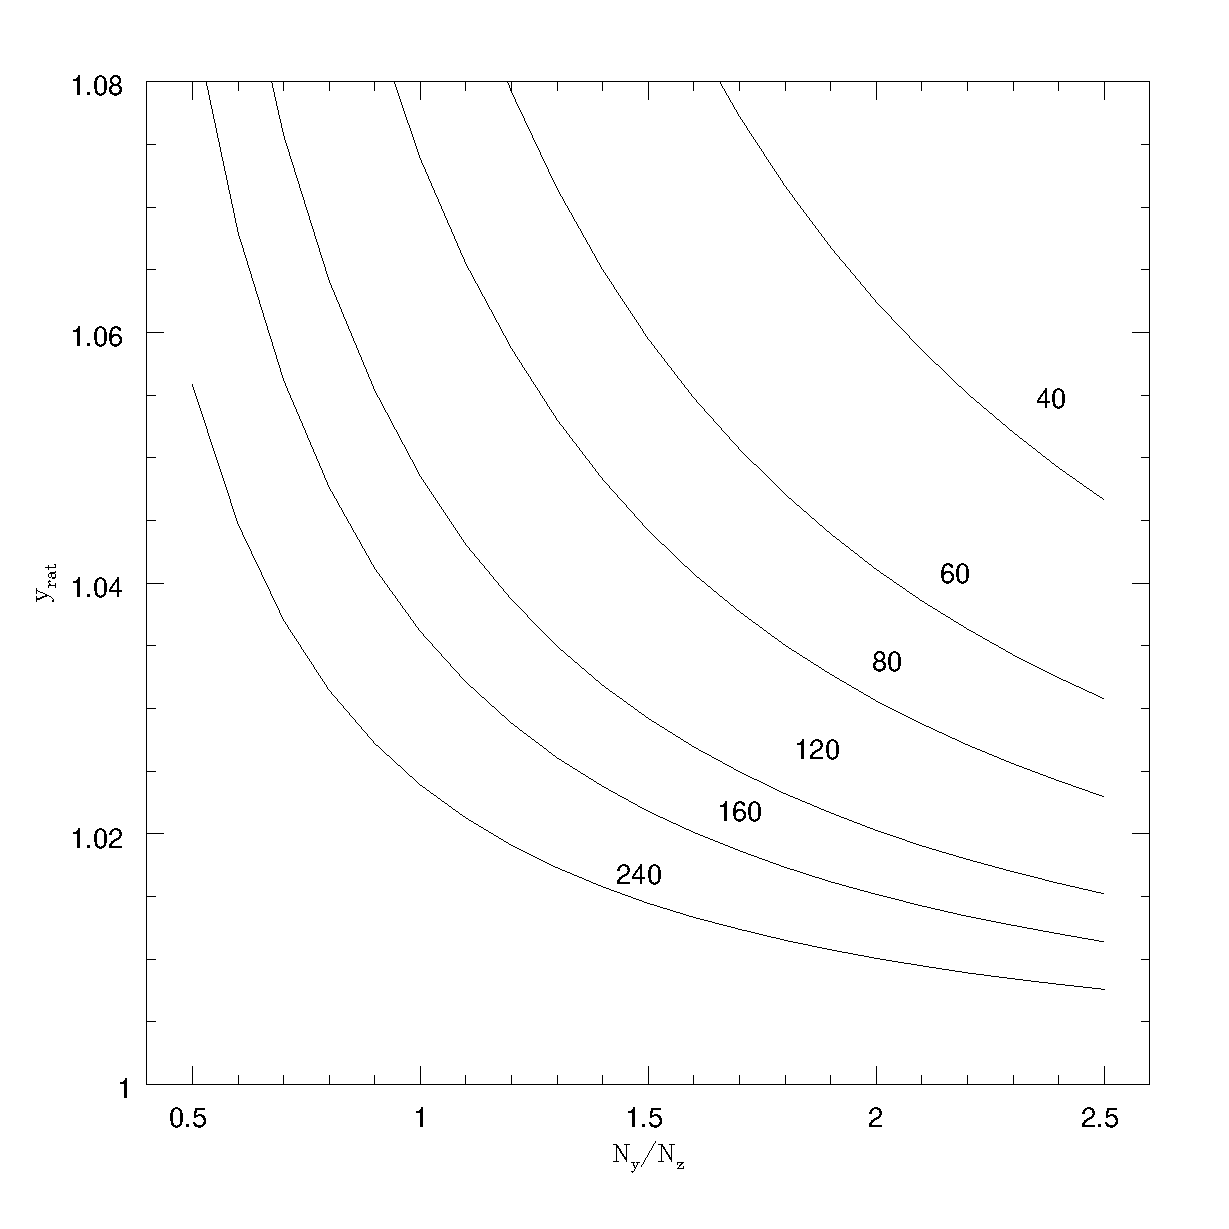
\includegraphics[width=3in]{yrat.ps}
\caption{The zone expansion factor, {\tt yrat}, as a function of
the ratio of radial to angular zones, for a few selected values
of the number of angular zones.
}
\end{figure}


\section{Output Files}

For the remainder of the discussion, we will assume all data produced
by {\tt cmhog} is dumped in a run-directory. In general, it is a good
idea to remove any potential files {\tt cmhog} may create, though
in practice only the {\tt hdfXXXbg} files are the problem makers
(by default data would be appended to any existing HDF files).

Depending on options given to the program, you may find the following files
in your run directory:

\begin{itemize}

\item
{\tt cmhogin}
Input namelist, that controls the program. This is generally
the only input file (except if pgrid is used, two fits files
will be input files).

\item
{\tt cmhogout}
Output namelist, reflects current state of all variables.

\item
{\tt history}
Ascii table with time in the first column, other columns 
are used for things such as mass loss across the inner and 
outer boundaries etc.etc.

\item
{\tt hdfXXXbg}
Full HDF dataset, in HDF4/SDS format (Scientific Data Set), typically
with three named ``fields'': the 
{\tt R-VELOCITY}, {\tt PHI-VELOCITY}, and {\tt DENSITY}.
The NEMO program {\tt tsd} will display the contents of
such SDS files. Each file contains information for one timestep.
{\tt hdf0000bf} is normally the first one, for $t=0$ at the beginning
of the simulation.
\newline
{\bf NOTE:} Existing dataset will get their new SDS's appended to
the previous ones. Most scripts that will be discussed in this
paper, will then break. 

\item
{\tt mdeXXXbg}
Sample X-Y gridded density in a 8bit deep image (if {\tt dtmovie} $>$ 0)

\item
{\tt mvrXXXbg}
Sample X-Y gridded radial velocity in a 8bit deep image (if {\tt dtmovie} $>$ 0)

\item
{\tt mvtXXXbg}
Sample X-Y gridded tangential in a 8bit deep image (if {\tt dtmovie} $>$ 0)

\end{itemize}

Although the author has mostly used NEMO for analysis and visualization, 
there is a native NCSA program which can be used to quickly just look
at the numbers.

\begin{verbatim}
  % hdp dumpsds -i <index> -d <hdf_file>
\end{verbatim}
which writes only the data of set with index 
{\tt index}.  Index 0 are the phi
values, index 1 are the radial values, and those are repeated in 3,4 and
6,7.  The v, w and d data is in sets 2, 5 and 8.  To get the dimensions,
use -h instead of -d on sets 0 and 1 to get the header (not the data) and
grep for the 'Size =' line.  Not all that pretty but it all works!
\begin{verbatim}
  % hdp dumpsds -i 0 -d hdf0001bg                 # PHI (vector)
  % hdp dumpsds -i 1 -d hdf0001bg                 # R (vector)
  % hdp dumpsds -i 2 -d hdf0001bg                 # R-velocity (matrix)
  % hdp dumpsds -i 5 -d hdf0001bg                 # PHI-velocity (matrix)
  % hdp dumpsds -i 8 -d hdf0001bg                 # DENSITY (matrix)
  
\end{verbatim}

\section{NEMO programs}

Most, if not all, NEMO programs come with a manual page that should
explain the command line parameters (keywords) in more detail.

\subsection{runcmhog}

{\tt cmhog} is a program that needs to be run in a clean directory, and you
cannot run another {\tt cmhog} in that directory. That is because the names
of files that {\tt cmhog} produces are FIXED by the program, and cannot be
changed even by the {\tt cmhogin} file (it is also not practical to do that).
To help running {\tt cmhog}, a small pre-processor was written, called
{\tt runcmhog}. It is a little C program available in NEMO with which you
can use a template {\tt cmhogin} file and override parameters and set
a run directory, e.g.

\begin{verbatim}
    % runcmhog -n cmhogin.small run001  aob=2.0
    % runcmhog -n cmhogin.small run002  aob=2.5
    % runcmhog -n cmhogin.small run003  aob=3.0
    % runcmhog -n cmhogin.small run004  aob=3.5
\end{verbatim}

Jianjun Xu (a student of Jim Stone) once wrote a nice graphical frontend,
based on Tcl/Tk, to parse and generate cmhogin files. The code still
exists, but has not been excersized in a long time.

\subsection{tsd}

{\tt tsd} scans an HDF SDS :
\footnotesize\begin{verbatim}
% tsd hdf0001bg 
Found 3 scientific data sets in run001/hdf0001bg
1: R-VELOCITY AT TIME=1.00E-01(20,37) km/sec  -> [740 elements of type: 5 (FLOAT32)]
2: PHI-VELOCITY AT TIME=1.00E-01(20,37) km/sec  -> [740 elements of type: 5 (FLOAT32)]
3: DENSITY AT TIME=1.00E-01(20,37) Msolar/pc**2  -> [740 elements of type: 5 (FLOAT32)]
\end{verbatim}\normalsize

but can also print out data values and the coordinate system. In our case, the
first axis is the radial coordinate, and will not be a regularly sampled axis. The
second axis is the angular coordinate, and will be regularly sampled
(normally between $-\pi/2$ and $\pi/2$).


\begin{figure}[htbp]
\centering
\subfigure[Polar coordinates]{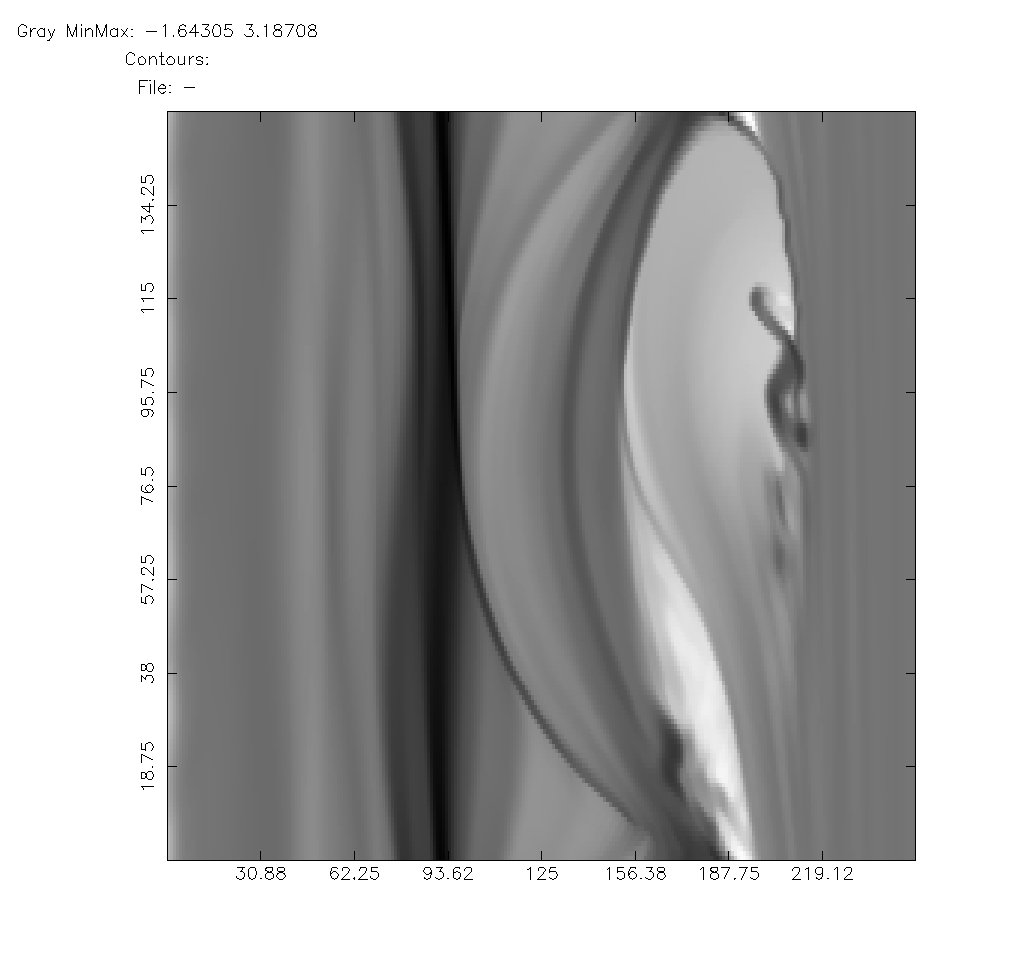
\includegraphics[width=2.2in]{denrt.ps}}
\hspace{0in}
\subfigure[Cartesian coordinates]{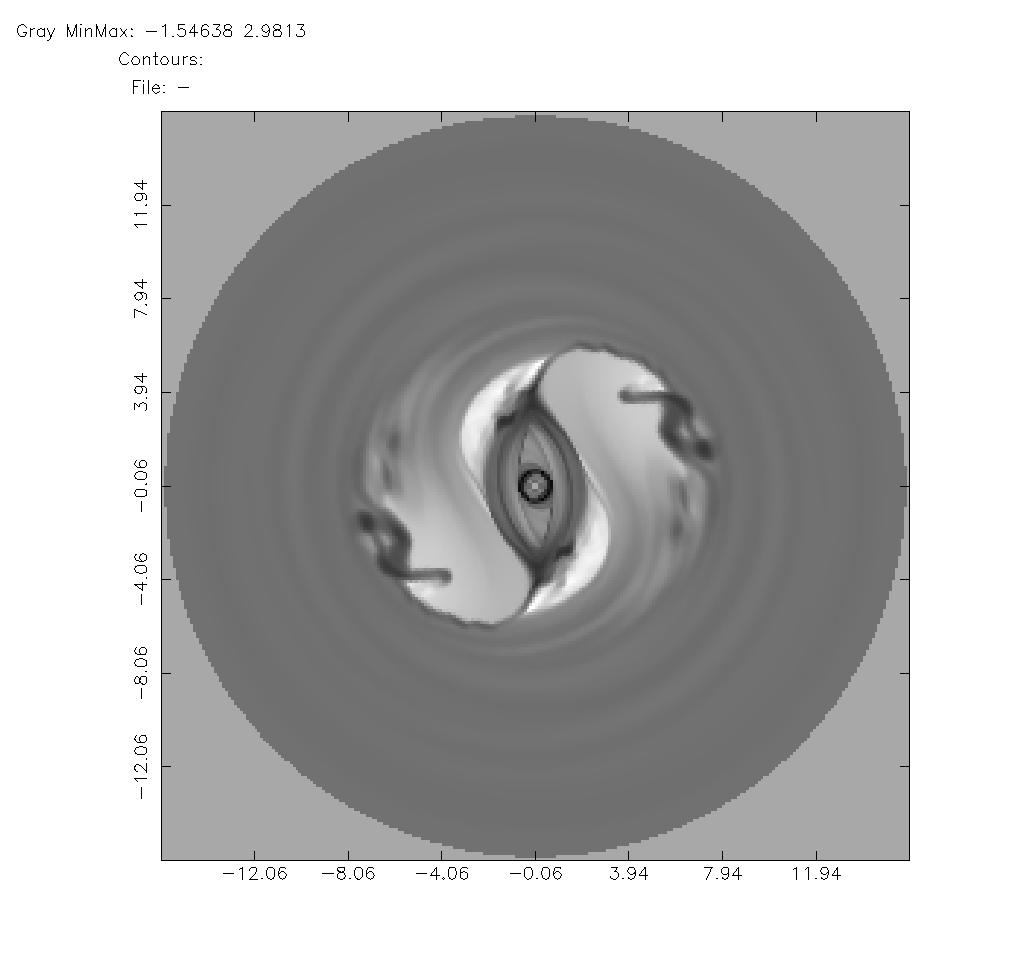
\includegraphics[width=2.2in]{denxy.ps}}
\caption{
Logarithmic density in polar coordinates:\newline
  \tt \% sdsfits hdf200bg mapd.fits 3\newline
  \tt \% fitsccd mapd.fits - | ccdmath - - 'log(\%1)' | ccdplot - yapp=denrt.ps/vps\newline
Logarithmic density in cartesian coordinates:\newline
  \tt \% hdfgrid hdf200bg - 3 | ccdmath - - 'log(\%1)' | ccdplot - yapp=den.ps/vps\newline
}
\end{figure}

Here is an example of getting the ``rotation curve'' from T=0. First we need to run
{\tt tsd} again, just to confirm how many radii we have, in this case the 2nd
dimension listed in the output of the arrays.

\footnotesize\begin{verbatim}

% tsd hdf0000bg
Found 3 scientific data sets in hdf0000bg
1: R-VELOCITY AT TIME=0.00E+00(40,67) km/sec  -> [2680 elements of type: 5 (FLOAT32)]
2: PHI-VELOCITY AT TIME=0.00E+00(40,67) km/sec  -> [2680 elements of type: 5 (FLOAT32)]
3: DENSITY AT TIME=0.00E+00(40,67) Msolar/pc**2  -> [2680 elements of type: 5 (FLOAT32)]
% tsd hdf0000bg - coord=t | head -67 | tabplot - 1 4

\end{verbatim}\normalsize


\subsection{sdsfits}

The individual ``fields'' from an {\tt hdfXXXbg} files can be converted to FITS files,
for visual inspection. Just remember that the first axis is the radial axis, the
second one the angular.  A ring will thus show up as a vertical structure.

\footnotesize\begin{verbatim}
% sdsfits hdf0001bg map001vr.fits 1
% sdsfits hdf0001bg map001vt.fits 2
% sdsfits hdf0001bg map001de.fits 3
\end{verbatim}\normalsize

Here is another plot:
\footnotesize\begin{verbatim}
% fitsccd mapd.fits - | ccdmom - - axis=2 mom=0 | ccdprint - x= newline=t | tabplot - 0 1 line=1,1
\end{verbatim}\normalsize
it plots total density averaged in rings, as function of cell.

\subsection{hdfgrid}

{\tt hdfgrid}
regrids selected gas properties from our 
HDF files into a cartesian coordinate system. 
It is specific to this polar-coordinate problem.

\footnotesize\begin{verbatim}
% hdfgrid hdf0001bg map000de.ccd zvar=den
% hdfgrid hdf0001bg map000vr.ccd zvar=vr
% hdfgrid hdf0001bg map000vt.ccd zvar=vt
% hdfgrid hdf0001bg map000vx.ccd zvar=vx
% hdfgrid hdf0001bg map000vy.ccd zvar=vy
\end{verbatim}\normalsize

Note that the {\tt vx} and {\tt vy} velocity fields
are computed on the fly. Nearest neighbor cells are
used for bi-linear interpolation. Some assumptions
about the symmetry properties of the variables
have been made, in case only a half-plane was
computed.



\section{flowcode}

Although gas flow in a barred galaxy never reaches an
exact steady state, it does approach something
that can perhaps be called a QSSS. However, another approach
to understand the gas flow is take a particular snapshot, and
integrate test particles in the velocity field, i.e.
solve the equations
$$
	{dx \over dt } = V_x(x,y)
$$
and
$$
	{dy \over dt } = V_y(x,y)
$$
NEMO's {\tt flowcode} program does that. For this a special
``vrt'' file (NEMO image format) is needed as input for the
integrator, consisting
of two 2D images with VR and VT, followed by two 1D images
with the coordinates in Radius and Polar Angle (called PHI)
A ``vrt'' map is created with a script {\tt mkvrt}.

\begin{verbatim}
In NEMO you will have to compile flowcode, e.g.

	mknemo flowcode

but also the .so files:

	cd $NEMO/src/nbody/evolve/flowcode
	make vrt.so vrtd.so
	cp *.so $NEMOOBJ/potential
		(sorry, no make target yet....)
	

The so-called ``vrt'' and ``vrtd'' files are to be made from HDF files,
with the script mkvrt and mkvrtd that didn't come with flowcode yet
...(catch-22)..

Here is an example of use: the initial conditions is gas flow on
circular orbits, so we'll integrate the flow and see if they remain
on circular orbits:

	mkvrt hdf0000bg test0000.vrt

\end{verbatim}

\subsection{NEMO scripts: mkbar}

Shell scripts are probably currently the easiest way to setup
problems. In order to make them reusable, much like NEMO
programs, they should take a series of {\it ``keyword=value''}
command line arguments.

\footnotesize\begin{verbatim}
#! /bin/csh -f
#
#
#> nemo.need mkconfig snapadd snapscale snaprotate snapspin

# bar length and axis ratio of bar
set b=1.4
set q=0.2

# 
set n=100

# derived quantities
set phi=`nemoinp "atand($q)"`

rm bulge line1 line2 bar disk model.dat

mkconfig - $n shell "$q*$b" | snapscale - bulge 1 1,1,0.4
mkconfig - $n line $b | snaprotate - -  90-$phi z | snapshift - line1 "-$q*$b,0,0"
mkconfig - $n line $b | snaprotate - - -90-$phi z | snapshift - line2 "$q*$b,0,0"
mkconfig - $n ring $b | snapscale - bar 1 $q,1,1
mkconfig - $n ring 2  | snapspin - disk 1
snapadd disk,bulge,line1,line2,bar model.dat 

\end{verbatim}\normalsize

\begin{figure}[htbp]
\centering
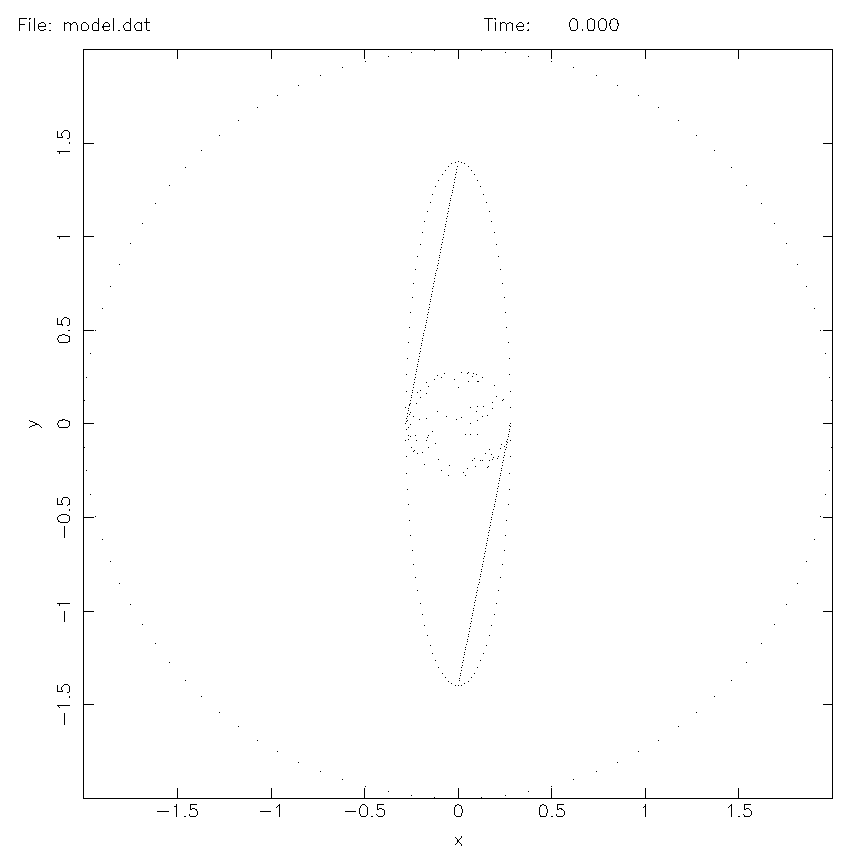
\includegraphics[width=3in]{model1.ps}
\caption{Face on view of a simple schematic for a counter-clockwise
rotating bar, as is used in the hydro models:\newline
 \tt \% snapplot model.dat yapp=model1.ps/vps
}
\end{figure}

\subsection{NEMO scripts: project}
 
Projecting a bar to match observations takes 3 geometric parameters:
position angle and inclination of the galactic disk, and position
angle of the bar. In addition there will be centering (xpos,ypos,vsys)
and scaling (pscale, vscale) parameters, that will come later. To
aid in figuring out the geometric projection, a script {\tt project}
was written, that projects the model from the previous section. It
is somewhat taylored for the way we measure angles in astronomy.

\footnotesize\begin{verbatim}
#! /bin/csh -f 
#
#> SCALE inc=0		0:90:1
#> RADIO rotation=ccw   ccw,cw
#> SCALE pa=0		-180:180:1
#> SCALE phi=0		-90:90:1
#> RADIO yapp=/xs       /xs,/vps,/ps
#> ENTRY text=  


foreach a ($*)
  set $a
end

if ($rotation == "cw") then
  snaprotate model.dat - "atand(tand($phi)/cosd($inc+180)),$inc+180,$pa" zyz |\
    snapplot - psize=vz/4 yapp=$yapp xlabel="inc=$inc ($rotation) pa=$pa phi=$phi" "ylabel=$text"
else
  snaprotate model.dat - "atand(tand($phi)/cosd($inc)),$inc,$pa+180" zyz |\
    snapplot - psize=vz/4 yapp=$yapp xlabel="inc=$inc ($rotation) pa=$pa phi=$phi" "ylabel=$text"
endif

\end{verbatim}\normalsize

This script uses NEMO's {\tt tkrun} interface, so you need to run it
as follows:

\footnotesize\begin{verbatim}
    % tkrun project
\end{verbatim}\normalsize

\subsection{NEMO scripts: mkbar\_cube\_ref.csh}

The script listed below is an older one where the geometry (cw/ccw) was not 
properly programmed, but included for completeness. It will use a reference
cube ({\tt n4303cube.fits}) to aid in matching up the theoretical data with
an observation.

\footnotesize\begin{verbatim}
#! /bin/csh -f
#
#  This scripts takes an HDF output snapshot file from cmhog
#  (bar hydro, polar coordinates), projects it to a requested
#  sky view, and using WIP summarizes the results
#  Bar is conveniently oriented along Y axis (PA=0), and flows CCW.
#  For CW rotating galaxies you may have to add 180 to 'inc' and/or 'pa'
#
#
#  23-sep-95	Created				Peter Teuben
#  15-nov-95    beam=0.2 frang=45
#  24-nov-95    defaults for more central region, fixed dependancies
#   9-jul-96    hacking for N5383 
#  24-jul-00    BIMA proposal N4303 et al.
#   5-sep-00    modified to write cubes instead of moment maps
#  12-mar-01    radecvel=t to make karma swallow these fits files
#  13-mar-01    use phi,inc,pa (no more +/- 180) and documented geometry
#               (notice that earlier versions had sign of radial vel wrong)
#  23-mar-01    added a refmap and fixed refscale; this assumes that the refmap
#		(often a cube) has the reference pixel defined to the be 
#		center of the galaxy (bimasong data often don't do the VELO axis correct)
#  17-apr-01    added velocity referencing using 'vsys' to be at v=0 in the model cube
#               (bugs when model and data have different delta-V)
#  11-apr-02    generic version with new geometry definitions

if ($#argv == 0) then
  echo Usage: $0 in=HDF_DATASET out=BASENAME ...
  echo Gridding and projecting 2D CMHOG hydro models to given bar viewing angles
  exit 0
endif

# 			Required Keywords
unset in
unset out
# 			Defaulted Keywords
set pa=-42
set inc=27
set phi=44
set rot=1
#
set rmax=6
set n=200
set beam=0.05
set color=1
set clean=1
#
set refmap=""
set pscale=0.5
set vscale=1
set vsys=0
#			Velocity gridding for cube  (dv=2*vmax/nvel)
set nvel=50
set vmax=250

set par=""

#			Parse commandline to (re)set keywords, special case for par=
foreach a ($*)
  set $a
  if (-e "$par") then
    source $par
    set par=""
  else
    echo Warning, par=$par does not exist
    set par=""
  endif
end

#
#  fix inc/pa for ccw(rot=1) or cw(rot=-1) cases for NEMO's euler angles
#
if ($rot == -1) then
   set inc=$inc+180
else if ($rot == 1) then
   set pa=$pa+180
else
   echo "Bad rotation, must be 1 (ccw) or -1 (cw)"
   exit 1
endif

#			Show i'm happy
echo Files: in=$in out=$out 
echo Grid: rmax=$rmax n=$n beam=$beam
echo Projection: phi=$phi inc=$inc pa=$pa
#                       Derived quantities
set cell=`nemoinp "2*$rmax/$n"`
set range="-${rmax}:${rmax}"
echo "      Derived: cell=$cell"

if (-e "$refmap") then
    #   referencing 
    set nz=(`fitshead $refmap | grep ^NAXIS3 | awk '{print $3}'`)
    set pz=(`fitshead $refmap | grep ^CRPIX3 | awk '{print $3}'`)
    set vz=(`fitshead $refmap | grep ^CRVAL3 | awk '{print $3}'`)
    set dz=(`fitshead $refmap | grep ^CDELT3 | awk '{print $3}'`)
    
    set dz1=`nemoinp "2000*$vmax/$nz"`
    set vref=`nemoinp "($vz-1000*$vsys)/($dz1)+$nvel/2+0.5"`
    #set vscale=`nemoinp "$vscale*(2*$vmax/$nvel)/($dz/1000)"`
    set refscale=$pscale,$pscale,$vscale
    #                                    CHECK : is this -0.5 or +0.5   ?????
    set refcen=`nemoinp $n/2-0.5`
    #set refpix=$refcen,$refcen,$vref

    
    #   now assuming model is centered, as well as data cube
    set vref=`nemoinp $nvel/2+0.5`
    ###set vref=`nemoinp $nvel/2-0.5`
    set refpix=$refcen,$refcen,$vref
    
    
    echo $nz $pz $vz $dz 
    echo Vsys at OBS pixel: `nemoinp "(1000*$vsys-$vz)/$dz+$pz"` 
    echo REFPIX:   $refpix
    echo REFSCALE: $refscale
else
    echo BUG: need to rewrite this section for when no refmap given..... since you did not
    exit 1
endif    

#> nemo.need tabtos snaptrans snaprotate snapadd snapgrid ccdsmooth ccdmath ccdfits fitshead

set tmp=tmp$$
if (! -e $out.den.fits) then

    # convert the half-plane HDF file to a full plane snapshot file

    tsd in=$in out=$tmp.tab coord=t
    if ($status) goto cleanup
    tabtos in=$tmp.tab out=$tmp.s0 block1=x,y,vx,vy,mass
    snaptrans in=$tmp.s0 out=$tmp.s1 ctypei=cyl ctypeo=cart
    snaprotate in=$tmp.s1 out=$tmp.s2 theta=180 order=z
    snapadd $tmp.s1,$tmp.s2 $tmp.s3

    # project for skyview, and create a intensity and velocity field

    snaprotate $tmp.s3 $tmp.snap \
        "atand(tand($phi)/cosd($inc)),$inc,$pa" zyz

    foreach mom (0 1 2)
         snapgrid in=$tmp.snap out=$tmp.$mom \
                xrange=$range yrange=$range nx=$n ny=$n moment=$mom mean=t
         ccdsmooth in=$tmp.$mom out=$tmp.$mom.s gauss=$beam
    end
    ccdmath $tmp.1.s,$tmp.0.s $tmp.vel %1/%2
## BUG: ifgt() doesn't work
##    ccdmath $tmp.0.s - "ifgt(%1,0,log(%1),-10)" | ccdfits - $out.den.fits
    ccdmath $tmp.0.s - "log(%1)" | ccdmath - - "ifeq(%1,0,-10,%1)" | ccdfits - $out.den.fits  \
        object=$in comment="$0 $in $out $pa,$inc,$phi,$range,$n,$beam"  \
	refmap=$refmap scale=$refscale refpix=$refpix
    ccdmath $tmp.2.s,$tmp.0.s,$tmp.vel - "sqrt(%1/%2-%3*%3)" | ccdfits - $out.sig.fits \
        object=$in comment="$0 $in $out $pa,$inc,$phi,$range,$n,$beam" 	\
	refmap=$refmap scale=$refscale refpix=$refpix
    ccdfits $tmp.vel $out.vel.fits \
        object=$in comment="$0 $in $out $pa,$inc,$phi,$range,$n,$beam" 	\
	refmap=$refmap scale=$refscale refpix=$refpix


### BUG:      ccdmath - - "ifgt(%1,0,log(%1),-10)" |\


    # now also create the (smoothed) cube
    snapgrid in=$tmp.snap out=- \
          xrange=$range yrange=$range zrange=-${vmax}:${vmax} \
	  xvar=x yvar=y zvar=-vz \
	  nx=$n ny=$n nz=$nvel moment=0 mean=t |\
      ccdsmooth - - gauss=$beam |\
      ccdmath - - "log(%1)" |\
      ccdmath - - "ifeq(%1,0,-10,%1)" |\
      ccdfits - $out.cube.fits \
        object=$in comment="$0 $in $out $pa,$inc,$phi,$range,$n,$beam" \
	refmap=$refmap scale=$refscale refpix=$refpix

    rm -fr $tmp.*
else
    echo Warning: skipping gridding and projecting
endif

exit 0

cleanup:
    if ($clean) rm $tmp.*





\end{verbatim}\normalsize



\section{cmhog: the Program}

Files are .src (fortran source to be pre-processed by cpp) and 
.inc (for the preprocessor) and .h (standard fortran includes).
On some operating systems (e.g. GNU/linux) the use of
{\tt cpp} as a pre-processor meant that single quotes could 
not be used in fortran comments.

\begin{verbatim}
    main    
        mstart
	    setup
	    grid_generator    (ggen)
	    problem_generator (galaxy)
	    nudt
        dataio
	
	solver
	intchk
	dataio
	special
	nudt
	
	dataio
\end{verbatim}

\subsection{Potential}

The potential and forcefield are defined through two subroutines
named {\tt inipotential} and {\tt potential}. They follow the
standard way how potentials are coded in the NEMO environment,
with the advantage that a variety of NEMO programs are now 
acccessible to investigate such potentials. Within NEMO potentials
can be written in either Fortran or C, although in order for
{\tt cmhog} to make use of them, any C version would need the
usual interface layer between Fortran and C. The standard distribution
of the bar hydro project of {\tt cmhog} implements the potential
in {\tt piner94.src}, which is (or should be) identical to the
one in {\tt \$NEMO/src/orbit/potential/data/piner94.f}.

The standard ``piner94'' potential is fixed in size by
setting the bar length to 5kpc and the velocity amplitude
at 20 kpc to 164.204 km/s (see discussion in Athanassoula 1992)

The following are the standard ``potpars'' parameters to this potential.

\begin{verbatim}
  omega           normally set to 0, since it is derived from ``lagrad'', and returned in this slot
  amode           not used [0]
  index           power of bar density law, not used ? [1]
  axirat          Axis ratio a/b of the bar (a number > 1) [2.5]
  radlag          Lagrangian radius along the bar axis, defined where the forces balance [6.0]
  quad            Quadrupole moment, measures the bar strength [45,000]
  cenden          Central Density, sets the slope of the central velocity field [24,000]
                  (or equivalently, the core radius)
  
\end{verbatim}

\subsection{Potentials on a grid}

In the fall of 2002 the {\tt cmhog} code was modified to handle potentials
on a grid. Two additive potentials, as FITS files, can be given in the
(new) {\bf pgrid} directive in the {\tt cmhogin} file. The coordinate
system in the FITS file, as defined by the usual CRVAL/CRPIX/CDELT keywords
in the FITS header, must be linear and in KPC (typically covering -16 to
16 kpc or so, but perhaps a little more to handle the edges). 

The following shell snippet shows how to create a potential:


\begin{verbatim}

% potccd grid0 athan92 0,1,1,2.5,6.5,0,24000 x=-17.5:17.5:0.07 y=-17.5:17.5:0.07 omega=0
% ccdfits grid0 grid0.fits 
% fitshead grid0.fits

SIMPLE  =                    T /
BITPIX  =                  -32 /
NAXIS   =                    3 /
NAXIS1  =                  501 /
NAXIS2  =                  501 /
NAXIS3  =                    1 /
COMMENT  FITS (Flexible Image Transport System) format is defined in 'Astronomy
COMMENT  and Astrophysics', volume 376, page 359; bibcode: 2001A&A...376..359H
CRPIX1  =      1.000000000E+00 /
CRPIX2  =      1.000000000E+00 /
CRPIX3  =      1.000000000E+00 /
CRVAL1  =     -1.750000000E+01 /
CRVAL2  =     -1.750000000E+01 /
CRVAL3  =      0.000000000E+00 /
CDELT1  =      7.000000030E-02 /
CDELT2  =      7.000000030E-02 /
CDELT3  =      0.000000000E+00 /
CTYPE1  = 'X       '           /
CTYPE2  = 'Y       '           /
CTYPE3  = 'Z       '           /
DATAMIN =     -2.563205781E+05 /
DATAMAX =     -4.864591797E+04 /
ORIGIN  = 'NEMO    '           /
AUTHOR  = 'teuben  '           /
OBJECT  = '        '           /
COMMENT
HISTORY  NEMO: History in reversed order
HISTORY  ccdfits grid0 grid0.fits VERSION=5.0
HISTORY  potccd grid0 athan92 0,1,1,2.5,6.5,0,24000 x=-17.5:17.5:0.07 y=-17.5:1
         7.5:0.07 omega=0 VERSION=1.4
END


\end{verbatim}



\section{Installation}

The best way to obtain {\tt cmhog} is via 
anonymous CVS\footnote{See {\tt http://www.astro.umd.edu/~teuben/miriad/cvs.html}
for more details on CVS usage}: 

\begin{verbatim}
	cvs -d :pserver:anonymous@cvs.astro.umd.edu:/home/cvsroot login
		(no password required, just hit ENTER)
	cvs -d :pserver:anonymous@cvs.astro.umd.edu:/home/cvsroot co cmhog2
		(this will create a cmhog directory)
	cd cmhog2
	configure --help              (study the options you may which to use, see below)
	configure
	make cmhog
	make bench

\end{verbatim}


\begin{verbatim}
% configure --help
...
Optional Features:
  --disable-FEATURE       do not include FEATURE (same as --enable-FEATURE=no)
  --enable-FEATURE[=ARG]  include FEATURE [ARG=yes]
  --enable-cfitsio        enable it, the default is that it won't use CFITSIO
 
Optional Packages:
  --with-PACKAGE[=ARG]       use PACKAGE [ARG=yes]
  --without-PACKAGE          do not use PACKAGE (same as --with-PACKAGE=no)
  --with-pgmax=SIZE          Maxim size grid that can be read with cfitsio
  --with-cfitsio-prefix=PFX  prefix where cfitsio lives (lib,include or sourse)
 
\end{verbatim}

If compilation still fails, e.g. due to the FITSIO interface, you may also manually need to edit
the Makefile to the correct path of where FITSIO (normally libcfitsio.a ) is located. Also
look at the cmhog.def file. Both files will be overwritten if you run {\tt configure} though, so
use the manual solution with care.


\newpage
\subsection{Benchmark}

The  {\tt cmhog} benchmark is defined as running the
standard PST95 model just through the bar growth time, 0.1Gyr,
on a small $67 \times 40$ grid (see {\tt cmhogin.bench}). This
benchmark uses about $4.41665e6$ zone cycles
The results for a few popular machines are summarized
in Table 1.

\begin{table}[htbp]
\centering
\medskip
\caption{{\tt cmhog} code benchmarks}
\begin{tabular}{|l|r|r|r|r|l|} \hline
Machine & MHz  	      
	& cpu(sec) 
	& cpu/GHz 
	& K-zcs\footnote{Kilo zone-cycle per second, computed as 4416.65/cpu(sec)}
	& compiler/options \\ 
&&&&&  \\ \hline
Intel i7 870    & 2930  &         5.22 &      & 4891  & g77 -g -O2 \\ % chara @ 2011
                &       &         4.76 &      & 442.  & \\
Core2Duo/T7300  & 2000  &        16.5 & 33.0  & 267.7 & gfortran -O2 \\  % nemo
P-IV/512        & 3000  &        13.4 & 40.2  &       & ifc -O2 \\  % kuma 
                &       &        10.4 & 31.2  & 423.5 & ifc -O2 -xW -tpp7 -ipo -i\_dynamic \\
P-IV/512	& 2800	&	 21.5 &       &       & g77 -g -O2 \\  % chand
                &       &        52.6 &       &       & -g \\
                &       &        14.3 &       &       & ifc -O2 \\    
P-IV/512	& 2200	&	 26.3 & 57.8  &  76.4 & g77 -g -O2 \\  % peto
                &       &        20.6 & 45.3  &  97.5 & ifc -O \\
		&       &        33.5 &       &       & ifc -O2 -mp \\
P-IV		& 2000  &	 29.4 & 58.8  &  75.1 &  \\  % magus
P-IV		& 1800  &	 32.4 & 58.3  &  75.8 &  \\  % juno, Harrington's machine
P-IV            & 1600  &        42.2 &       & 104.6 & g77 -g -O2 \\ % nemo laptop
AMD 		& 1600  &        23.1 & 37.0  & 119.4 & \\ % ithil
                &       &        17.6 & 28.2  & 156.6 & ifc -O \\
P-III Coppermine & 933   &	 56.6 & 52.8  &  83.6 & \\ % grus
                 &       &       40.8 & 38.1  & 115.9 & ifc -O \\
P-III		& 700   &	 75.2 & 52.6  &  84.0 & \\ % akash
P-III/512 Katmai & 600	&	 88.7 & 53.2  &  83.0 &  \\ % mensa
P-III		& 600	&	 91.1 & 54.7  &  80.7 & (laptop) \\ % laptop
 		& 	&	 65.0 & 39.0  & 113.2 & ifc -O \\
		&	&	 70.8 &       &       & pgf77 -O (version 3.2) \\
		&	&	 93.6 & 56.2  &  78.6 & ifc -O compiled on Piv \\
P-III/512 Katmai & 500  &	106.5 & 53.3  &  82.9 & \\  % xeon (P500 at home)
                &       &        89.5 & 44.3  &       & gcc 3.2.2 @ mdk91 \\
P-II/MMX        & 233   &       321.0 & 74.8  &  13.7 & g77 -g -O2 \\ % peter(P233MMX at home)
		&	&	321.6 & 74.9  &  13.7 & ifc -O \\
P-I             & 166   &       496.1 & 82.4  &   8.9 & g77 -g -O2 \\ % saturn
\hline
G4              & 1400  &        29.7 &       & 148.8 & g77 -g -O2\\ % peter's summer G4  (26.9 if spamp=0)
G4              &  800  &        60.5 & -     &  79.9 & g77 -g -O2 \\ % eve's laptop
\hline
Alpha EV67	& 666   &        42.7 & 28.4  & 103.4 & g77/gcc \\ % numenor
		&       &        23.8 & 15.8  & 185.5 & fort/ccc -fast \\
Ultra-SPARC-IIi &  440  &	   -  &   -   &       & g77 -g -O2\\   % venus
		&  	&	 66.0 & 29.0  &  66.9 & f77 -O \\
		&  	&	 55.0 & 24.2  &  80.3 & f77 -fast  ?? \\
		&	&	 44.0 & 19.4  & 100.4 & f77 -fast \\
Ultra-SPARC     &  167  &       128.0 & 21.4  &  34.5 & f77 -fast \\
 \hline
\end{tabular}
\end{table}
%% \end{minipage}

%  full tests on P2200:
%  20 80.3
%  40 445.4
%  80 3193.8    gcc=run007 4581 w/gcc
% A few ``2002'' comments:
\begin{itemize}
\item An Ultra-SPARC is about twice as efficient as an Intel chip.

\item The Pentium-iii is about 10-15\% more efficient per clock cycle
than the Pentium-iv.

\item The Intel compiler is about 30-40\% more efficient compared
to the GNU compiler (and it doesn't matter if this is on an intel or AMD chip)

\item There is no benefit from using a 512kB cache size 

\item The Alpha is the most efficient processor per clock cycle (native compiler)

\item Piv code running on a Piii chip will slow down the code considerably

\item Compiler version can make a big difference

\end{itemize}

\begin{verbatim}
ratio of gnu to intel compiler on a Piv/2.2

 nphi    gnu    intel
  20    4.10     3.31
  40   26.43    21.08
  80  201.9    161.32
 154

\end{verbatim}

\end{document}

\footnotesize\begin{verbatim}
\end{verbatim}\normalsize


\begin{verbatim}
\end{verbatim}






